\documentclass[runningheads,a4paper]{llncs}

\usepackage{amssymb}
\setcounter{tocdepth}{3}
\usepackage{graphicx}
\usepackage{calc,listings,color}

\usepackage[ruled,nothing]{algorithm}
\usepackage{algorithmic}
\renewcommand{\algorithmicrequire}{{\textbf{Input:}}}
\renewcommand{\algorithmicensure}{{\textbf{Output:}}}

\usepackage{url,xspace}

\newcommand{\linboxsp}{{\sc LinBox}\xspace}
\newcommand{\linbox}{{\sc LinBox}}

\begin{document}

\mainmatter  
\title{\linboxsp scope allocation, parallel building blocks and
  separate compilation models}
%\titlerunning{}

\urldef\jgdemail\url{Jean-Guillaume.Dumas@imag.fr}
\urldef\cpemail\url{Clement.Pernet@imag.fr}
\urldef\bdsemail\url{saunders@cis.udel.edu}
\urldef\tgemail\url{Thierry.Gautier@inrialpes.fr}

\author{
Jean-Guillaume Dumas\inst{1}
\and Thi\'erry Gautier\inst{2}
\and Cl\'ement Pernet\inst{2}
\and B. David Saunders\inst{3}
}

\institute{
Laboratoire J. Kuntzmann, Universit\'e de
Grenoble. 51, rue des Math\'ematiques, umr CNRS 5224, bp 53X, 
F38041 Grenoble, France, \jgdemail.
\and
Laboratoire LIG, Universit\'e de Grenoble. umr CNRS, 
F38330 Montbonnot, France. \cpemail, \tgemail.
\and University of Delaware, Computer and
  Information Science Department. 
Newark / DE / 19716, USA. \bdsemail.}

\maketitle

\section{Introduction}

As a building block for a wide range of applications, computational exact linear
algebra has to conciliate both efficiency and genericty. The goal of the 
\linboxsp project is to address this problem by designing an efficient general-purpose
\texttt{C++} open-source library for exact linear algebra over the integers, the
rationals and finite fields. 
Matrices can be either dense, sparse or black box (i.e. viewed as a linear
operator, acting on vectors only). The library proposes a set of high level
linear algebra solutions, such as the rank, the determinant, the solution of a
linear system, the smith normal form, the echelon form, the characteristic
polynomial, ... Each of these solutions involve a hybrid combination of several specialized
algorithms depending on the domain, and the type of matrix. Over a finite field,
the building blocks are an efficient implementation of Wiedemann and block
Wiedemann algorithms combined with preconditioners~\cite{CEKSTV:2002:EP} for
black box matrices, a sparse Gaussian elimination for sparse matrices and the
BLAS based dense linear algebra techniques of the \texttt{FFLAS}
library~\cite{DGP:2008:dlaff} for dense matrices. The solutions over the integers
and rationals are lifted from modular computations by a Chinese remainder
algorithm or $p$-adic lifting.
The design based on a high genericity allow to write efficient algorithms  independently from the
representations of domains and matrices. As a middleware, the library relies on the
efficiency of kernel libraries such as  \texttt{GMP}\footnote{\url{http://gmplib.org/}},
\texttt{Givaro}\footnote{\url{http://www-ljk.imag.fr/CASYS/LOGICIELS/givaro/}},
\texttt{NTL}\footnote{\url{http://www.shoup.net/ntl/}},
\texttt{ATLAS}\footnote{\url{http://math-atlas.sourceforge.net/}} and can be used by general
purpose computer algebra systems such as \texttt{Sage}\footnote{\url{http://sagemath.org/}} or \texttt{Maple}\footnote{\url{http://www.maplesoft.com/}}. 

\section{A lightweight memory management}

\subsection{Call-by-reference}

Only references as argument (no value returned), first args as return
values.

\verb! Matrix & Function( Matrix & result, const XXX& args); !

example of fields \cite[\S 2.1]{jgd:2002:icms} ?

\subsection{The mother model}


The mother model: functions should not allocate their return values

\begin{itemize}
\item more efficient: allocations are limited

\item requires more involvment by the programmer: control of the allocation

\item garbage collection is simplified: reference counting with a single
boolean, or even better (sic) by two different classes.
Especially for thread-safety.
\end{itemize}


\subsection{Rebind of matrices}

mecanism of the rebind for fields adapted from STL rebind of
allocators.

Since rebind must not allocate, only references are given (re)
allocation is done by the caller (and not rebind), rebind only maps
values from one field to another.

\begin{itemize}
\item generic homomorphism 
\verb!e.init( newelt, e.convert( Integer, oldelt) )!
can be specialized.
\end{itemize}

\section{Software abstraction layer for parallelism}

Efficient parallel applications must take into consideration hardware
characteristics (number of cores, memory hiearchy, ...): it is time
consuming or impossible for a single developer to be able to
program a high performance computer algebra application, with state of
the art algorithm, that will exploit all the available parallelism.  
In order to separate the domain of expertise we have designed a
software abstraction layer between computer algebra algorithms
and parallel implementations, with automatic dynamic scheduling.

\subsection{Parallel building blocks}
Computer algebra algorithms have three main characteristics:
\begin{enumerate}
\item They are complex and require a deep knowledge of the problem in
  order to the most efficient sequential algorithm.
\item They may be highly irregular. This enforce a runtime usage of
  load balancing algorithms.
\item They are generic in the sense that it they are usually designed
  to work generically over several input domains.
\end{enumerate}

  In the case of \linboxsp algorithms, we have decided to base our
  software abstraction, called {\em Parallel Building Blocks (PBB)},
  on the STL algorithms (Standard Template Like) principles.

  Indeed, C++ data structure in \linboxsp let us to have random access
  iterators over containers which are naturally parallel. 
  
  We have already defined several algorithms STL-like and the list
  will be extended in the near future:
  \begin{description} 
    
  \item [for\_each, transform, accumulate \cite{Musser:1996:STL}:] the parallel building
    blocks for these three algorithms are similar to the STL version 
    except that the involved operators (or function class) given in
    parameter are required to have their return value passed by the
    first parameter of the function. 
    This is mainly due to the memory model of \linboxsp, since objects
    returned by these operator may have a large size (\textit{e.g} a
    matrix).
    Therefore, the STL return-by-value semantic is not appropriate. 
  \end{description} 
  
  Note that within the incoming C++0X standard, the lambda capability
  of the core language will simplify the use of these operators and
  therefore of the parallel
  building blocks.

%\verb!transform!, etc. 

%\begin{itemize}
%\item Transparent parallelism
%\item Abstraction of parallelism
%\item Parallelism really as a plug-in
%\end{itemize}
  
  The fundamental idea of these blocks is that at the computer algebra
  level, the parallelization of all the loops and more generally of all
  the STL-like algorithms will already enable:
\begin{enumerate}
\item Good performance: in many complex or irregular computer algebra
  applications this coarse-grain parallelization of the inner loops of
  the underlying linear algebra is sufficiently refined.
\item Different implementations of the parallel blocks: this
  abstraction allows for both a programming independent of the
  parallel model and an evolution of the parallel environment
  depending on the target architecture.
\end{enumerate}

The parallel blocks can be implemented using many different parallel
environments, such as OpenMP
\cite{Chapman:2007:openmp}; TBB (Thread Building Blocks)
  \footnote{\url{http://www.threadingbuildingblocks.org}} or
  Kaapi~\cite{inproceedingsgautier.gbp_ktsrsf_07}; using
  both static or dynamic work-stealing
  schedulers~\cite{con-traore.trmgb_08}.
The current implementation supports both OpenMP and Kaapi.

\subsection{Accumulate-while and early termination}
To bound the complexity of many linear algebra problems, one of the
key idea is to use an accumulation with {\em early termination}.

For instance, this is used in Chinese Remaindering algorithms: the
computation is performed modulo a sequence of (co)prime numbers and
the result is built from a sequence of residues, {\em only while} a
condition is satisfied~\cite{jgd:2010:crt}. 
The termination of the algorithm depend on the accumulated (here
reconstructed) result.
  
In order to parallelize such algorithms, we proposed an extension of
the STL algorithms called \verb+accumulate_while+:
\begin{description} 
\item [accumulate\_while:] The algorithm takes an array $v$, an
  operator $f$, an operator $+$ for the summation, and condition
  operator.
  For a sequence $S_k = \sum_{i=0,..,k} f( v[i])$ with 
  $k \in \{0,N\}$, the algorithm computes and returns $n$ and $S_n$ such that 
  $S_k, k \leq n$ does satisfy the condition and $S_k, k > N$
  may not satisfy this condition.
\end{description} 

  This algorithm is used 
  for the early termination Chinese remaindering algorithms of
  \linbox. A sequential version and parallel versions with OpenMP and
  Kaapi can be found in the \linboxsp distributions as 
  \url{linbox/algorithms/cra-domain-*.h}.

%\verb!Accumulate-while!, generalization of \cite{jgd:2010:crt},
%specially adapted to early termination in mathematical softwares.
%Other applications (e.g. from \cite{Beaumont:2004:PMAA}) ??


\subsection{Memory contention and thread safe allocation}
Many computer algebra programs allocate dynamic memory for the
intermediate computations. Several experiments with \linboxsp
algorithms, on multicore architectures, have shown that these
allocations are quite often the bottleneck in the performance.

An analysis of the memory pattern and experimentations with three well
known memory allocators 
(ptmalloc, Hoard and TCMalloc from Google Perf. Tools~\cite{tcmalloc})
have been conducted. The goal was to decide wether the parallel
building blocks model was suitable to high-performance exact linear
algebra.

Preliminary experiments on the Chinese remaindering {\bf accumulate\_while},
not the easiest to parallelize, have demonstrated the advantage, in
our setting, of TCMalloc over the others~\cite{jgd:2010:crt}.
One of the main reason for that fact is that our problems required
many temporary allocations. This fits precisely the thread safe caching
mechanism of TCMalloc.

\section{Automated Generic Separate compilation}
\linboxsp is developped with several levels of genericity:
\begin{itemize}
\item Genericity with respect to the domain of the coefficients;
\item Genericity with respect to the data structure of the matrices;
\item Genericity with the intermediate algorithms;
\item ...
\end{itemize}
While efficient in terms of capabilities and code reusability, this
can lengthen the compilation time and generate large executable files.\\
For the management of code bloat \linboxsp proposes an ``archetype
mecanism'' which enable, at the user latitude, to switch to a
compilation against abstract classes \cite[\S 2.1]{jgd:2002:icms}.\\
This can reduce the efficiency of the library. Therefore, we propose
here a way to provide a generic separate compilation. This will not
deal with code bloat, but will reduce the compilation time while
preserving the performances.\\
This is useful for instance when the library is used with
unspecialized calls. This is largely the case for some interface
wrappers to other Computer algebra systems such as {\sc Sage} or {\sc Maple}.\\
Our idea is to automatize the technique of
\cite{Erlingsson:1996:issac} which combines compile-time instantiation
and link-time instantiation, while using template instantiation
instead of void pointers.\\
The mecanism we propose is independent of the desired method, candidate
for separate compilation and is explained on algorithm \ref{alg:sep}.
\begin{algorithm}[ht]
\caption{C++ Automatic separate compilation wrapping}\label{alg:sep}
\begin{algorithmic}[1]
\REQUIRE A generic function \texttt{func}.
\REQUIRE Some template parameters for separate specialization and
compilation of  \texttt{func}.
\ENSURE A generic function calling
\texttt{func} with separately compiled instantiations.
\STATE Create a header and a body files ``func\_instantiate.hpp'' and ``func\_instantiate.cpp'';
\STATE Add a template function \texttt{func\_separate}, with the same
specification as \texttt{func}, to the header;
\STATE Its generic default implementation is a single line calling the
original function \texttt{func}.\\ \COMMENT{This enables to have a
  unified interface, even for non specialized class.}
\FOR{each separately compiled template parameter \texttt{TParam}}
  \STATE Add  a non template specification
  \texttt{funcTParam}, to the header file;
  \STATE Add the associated body with a
  single line returning the instantiation of
  \texttt{func} on a parameter of type \texttt{TParam}, to the body file;
  \STATE Add an inline specialization
  body of \texttt{func\_separate} on a parameter of type
  \texttt{TParam} with a single line returning \texttt{funcTParam}, to
  the header file; 
\ENDFOR
\STATE Compile the body file ``func\_instantiate.cpp''.
\end{algorithmic}
\end{algorithm}

This Algorithm is illustrated on figure \ref{fig:sep}, where
the function is the \texttt{rank} and the template parameter is a dense
matrix over the finite field with two elements,
\texttt{DenseMatrix<GF2>}.
\begin{figure}[ht]
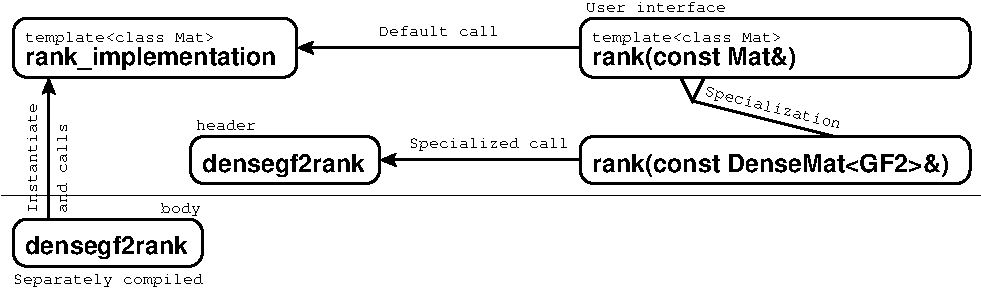
\includegraphics[width=\textwidth]{separate}
\caption{Separate compilation of a rank specialization}\label{fig:sep}
\end{figure}

We show on table \ref{tab:compilation} the gains, in term of compilation time,
obtained on two examples of \linbox: the \texttt{examples/rank.C} and
\texttt{examples/solve.C} algorithms. Indeed without any specification
the code
has to be generic and to invoke several specializations depending on
run-time discovered properties of thei input. For instance the
\texttt{solve.C} example requires at least 6 specializations for sparse
matrices over the Integers or over a prime field, with a sparse
elimination, or an iterative method, or a dense method if the matrix
is small, or an hybrid method...\\ 
\begin{table}[ht]\center
\begin{tabular}{|l||r|r|r||r|r|r|}
\hline
file                      &  real time   &  user time   &  sys. time  &  real time   &  user time   &  sys. time \\
\hline
 & \multicolumn{3}{|c||}{Rank}& \multicolumn{3}{|c|}{Solve}\\
\hline
\texttt{instantiate.o} & 143.43s & 142.47s & 0.90s & 171.62s & 170.42s & 1.12s\\
\texttt{separate.o} & \bf 18.58s & \bf 18.26s & \bf 0.30s & \bf 23.13s & \bf 22.80s & \bf 0.32s\\
\texttt{separate} & 0.80s & 0.64s & 0.15s & 0.85s & 0.70s & 0.14s\\
\hline
\texttt{Sep. comp.} & 162.81s & 161.37s & 1.35s & 195.60s & 193.92s & 1.58s\\
\hline
\texttt{Full comp.} & 162.02s & 160.47s & 1.21s & 191.47s & 189.52s & 1.40s\\
\hline
\hline
\texttt{speed-up} & 8.4 & 8.5 & 2.7 & 8.0 & 8.1 & 3.0s\\
\hline
\end{tabular} 
\caption{linbox/examples/\{rank,solve\}.C compilation time on an AMD
  Athlon 3600+, 1.9GHz, with gcc 4.5 -O2. \texttt{instantiate.o} corresponds to the separately compiled
  instantiatiations (e.g. densegf2rank in figure \ref{fig:sep});
  \texttt{separate.o} corresponds to the user interface and generic
  implementation compilation; \texttt{separate} corresponds to the
  linking of both \texttt{.o} and the library.}\label{tab:compilation}
\end{table}

\begin{remark} Algorithm \ref{alg:sep} has been simplified for the
  sake of clarity. To enable a more user-friendly interface and to
  leave it unchanged, one has to do two additional tasks:
\begin{enumerate}
\item Add a generic default implementation to \texttt{func\_separate}:
 with a single line calling the orginal function \texttt{func}. This
 enables to have a unified interface, even for non specialized class.
\item Rename the original function and all its
  original specializations \texttt{func\_original}; then rename also
  the new interface simply \texttt{func}. This allows to keep the same
  interface.
\end{enumerate}
\end{remark}

\begin{remark} 
With the classical inline compiler optimizations, the overhead of
calling \texttt{rank\_separate} is limited to single supplementary
function call. Indeed all the one line additionnal methods will be
automatically inlined, except, of course, the one calling the separately
compiled code.
If this overhead is nonetheless too expensive, it suffices to enclose all the non generic specializations of
``func\_instantiate.hpp'' by a macro test. 
At compile time, the decision to separately
compile or not can be taken according to the definition of this
macro. 
\end{remark}

\section*{Acknowledgment}
We thank the \linboxsp group and especially Brice Boyer, Pascal Giorgi,
Erich Kaltofen, Dan Roche, Brian Youse for many useful discussions 
in particular during the recent \linboxsp developer meetings in
Delaware and Dublin.


\bibliographystyle{plain}
\bibliography{icms} 

\end{document}
